\documentclass[12pt,a4paper]{article}
\usepackage[utf8]{inputenc}
\usepackage{amsmath}
\numberwithin{equation}{section}
\usepackage{amsfonts}
\usepackage{amssymb}
\usepackage{graphics}
\usepackage{graphicx}
\usepackage{xcolor}
\usepackage{tcolorbox}
\usepackage{tensor}
\usepackage{cancel}
\usepackage{dsfont}
\usepackage{rotating}
\usepackage{changepage}
\usepackage[left=2cm,right=2cm,top=2cm,bottom=2cm]{geometry}
\usepackage[nottoc]{tocbibind}
\usepackage{mathpazo}
\usepackage{hyperref}
\usepackage{float}
\usepackage{wrapfig}
\usepackage{fancybox}
\usepackage{tikz}
\usepackage{ragged2e}
\usepackage{lipsum}
\usepackage[explicit]{titlesec}
\usepackage{fancyhdr}
\usepackage{empheq}
\definecolor{myblue}{rgb}{.8, .8, 1}
\newcommand*\mybluebox[1]{%
\colorbox{myblue}{\hspace{1em}#1\hspace{1em}}}

%\newenvironment{rcases}
%  {\left.\begin{aligned}}
%  {\end{aligned}\right\rbrace}


\author{}
\date{}
\renewcommand*\contentsname{\textsc{CONTENTS}}
\renewcommand\thesection{\arabic{section}}
\renewcommand\thesubsection{\thesection.\arabic{subsection}}

%\usepackage{titlesec}
%
%
\colorlet{sectitlecolor}{blue!50!black}
%\colorlet{sectboxcolor}{blue!50!black}
\colorlet{secnumcolor}{white}
%\titleformat{\section}
%  {\normalfont\Huge\bfseries\color{sectitlecolor}}{\Huge\colorbox{sectboxcolor}{\Huge\textcolor{secnumcolor}{\thesection}}}{0.5em}{}





\colorlet{sectcolor}{blue!60!black}

\newcommand\graysquare{\textcolor{sectcolor}{\rule{1ex}{1ex}}}
\newcommand{\helv}{\fontfamily{phv}\fontseries{}\fontsize{10}{12}\selectfont}

\pagestyle{fancy}

%\renewcommand{\chaptermark}[1]{\markboth{#1}{}}
\renewcommand{\sectionmark}[1]{\markright{\thesection.\ #1}}
\fancyhf{}
\fancyhead[RO]{\helv\rightmark\hspace{0.5em}\graysquare\hspace{0.5em}\thepage}
\fancyhead[LE]{\helv\thepage\hspace{0.5em}\graysquare\hspace{0.5em}\leftmark}
\renewcommand{\headrulewidth}{0pt}

\titleformat{\section}
  {\normalfont\Huge\bfseries\color{sectitlecolor}}
  {\llap{\colorbox{sectcolor}{\makebox[20em][r]{\textcolor{secnumcolor}  {\thesection}}}\hspace{1em}}}
  {0em}{#1}

\titleformat{\subsection}
  {\normalfont\Large\bfseries\color{sectitlecolor}}{\thesubsection}{0.5em}{#1}
\titleformat{\subsubsection}
  {\normalfont\large\bfseries\color{sectitlecolor}}{\thesubsubsection}{0.5em}{#1}



\begin{document}

%----------------------------------------------------------------------------------------
%	TITLE PAGE
%----------------------------------------------------------------------------------------

\begin{titlepage} % Suppresses displaying the page number on the title page and the subsequent page counts as page 1
	\newcommand{\HRule}{\rule{\linewidth}{0.5mm}} % Defines a new command for horizontal lines, change thickness here
	
	\center % Centre everything on the page
	
	%------------------------------------------------
	%	Headings
	%------------------------------------------------
	
	\textsc{\LARGE Georg-August-Universität Göttingen}\\[1.5cm] % Main heading such as the name of your university/college
	
	\textsc{\Large Institut für Theoretische Physik
}\\[0.5cm] % Major heading such as course name
	
	\textsc{\large M.Phy.1403 - Report}\\[0.5cm] % Minor heading such as course title
	
	%------------------------------------------------
	%	Title
	%------------------------------------------------
	
	\HRule\\[0.4cm]
	
	{\huge\bfseries Helicity 2 Couplings to Matter Fields}\\[0.4cm] % Title of your document
	
	\HRule\\[1.5cm]
	
	%------------------------------------------------
	%	Author(s)
	%------------------------------------------------
	
	\begin{minipage}{0.4\textwidth}
		\begin{flushleft}
			\large
			\textit{Author}\\
			Ayush Paliwal % Your name
		\end{flushleft}
	\end{minipage}
	~
	\begin{minipage}{0.4\textwidth}
		\begin{flushright}
			\large
			\textit{Supervisor}\\
			Prof. Dr. Karl-Henning Rehren % Supervisor's name
		\end{flushright}
	\end{minipage}
	
	% If you don't want a supervisor, uncomment the two lines below and comment the code above
	%{\large\textit{Author}}\\
	%John \textsc{Smith} % Your name
	
	%------------------------------------------------
	%	Date
	%------------------------------------------------
	
	\vfill\vfill\vfill % Position the date 3/4 down the remaining page
	
	{\large\today} % Date, change the \today to a set date if you want to be precise
	
	%------------------------------------------------
	%	Logo
	%------------------------------------------------
	
%	\vfill\vfill
%	\begin{figure}[H]
%\centering
%\begin{minipage}{.5\textwidth}
%  \centering
%  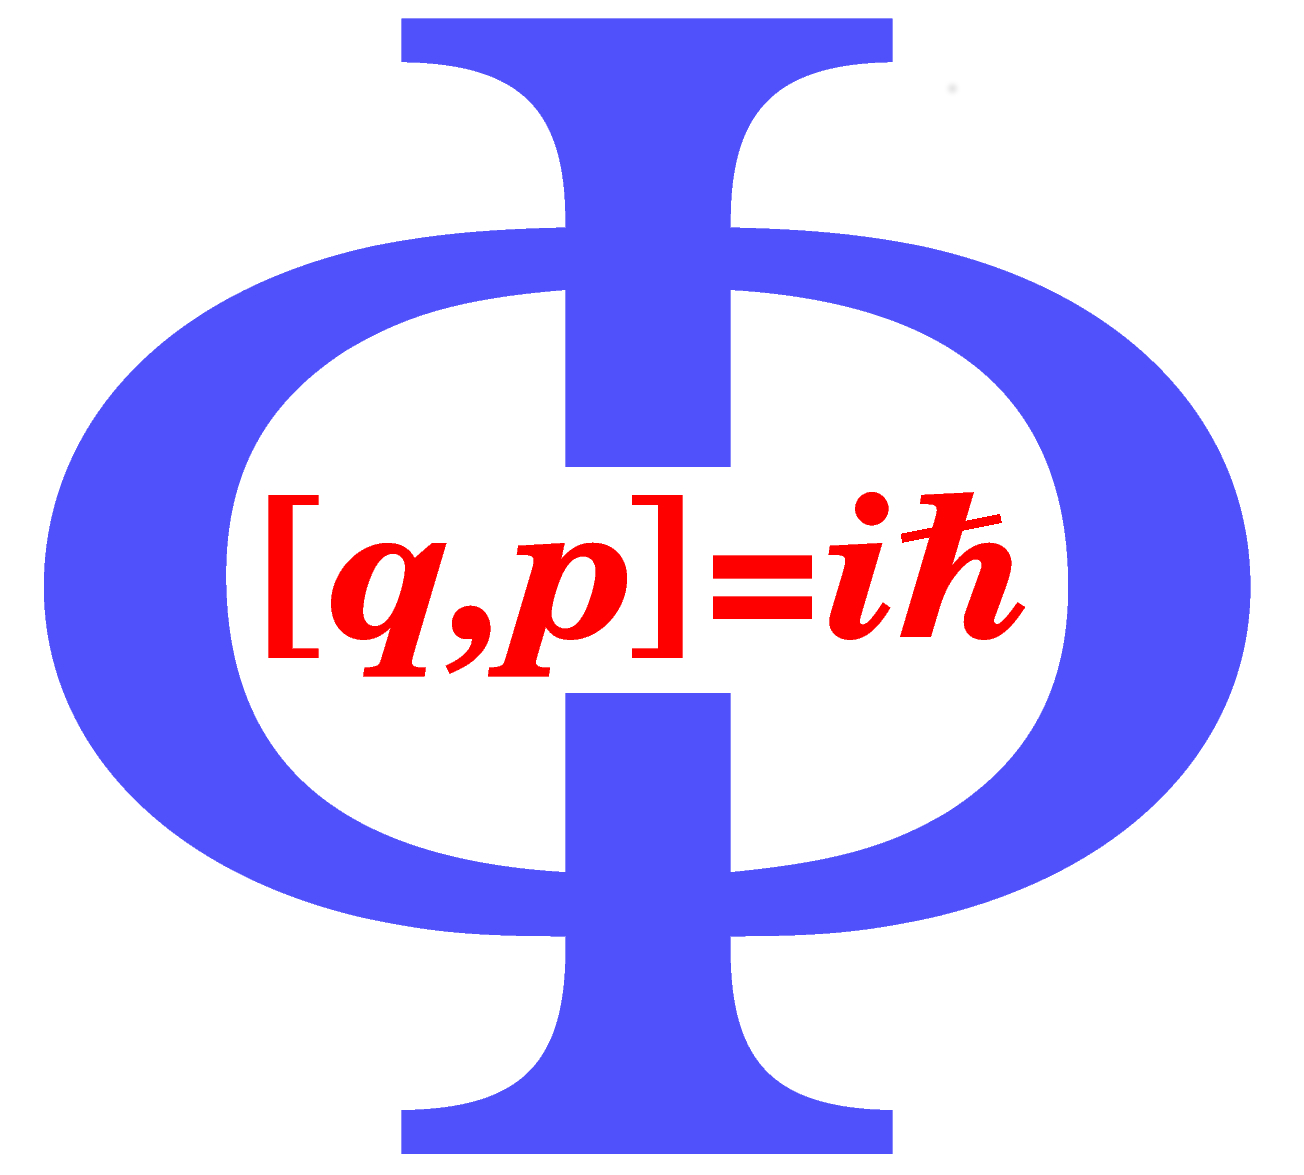
\includegraphics[width=.4\linewidth]{ITPlogo}
%  \label{fig:test1}
%\end{minipage}%
%\begin{minipage}{.5\textwidth}
%  \centering
%  
\includegraphics[height=0.25\linewidth, width=1\linewidth]{Unilogo}
%  \label{fig:test2}
%\end{minipage}
%\end{figure} % Include a department/university logo - this will require the graphicx package
	 
	%----------------------------------------------------------------------------------------
	
	\vfill % Push the date up 1/4 of the remaining page
	
\end{titlepage}

%----------------------------------------------------------------------------------------
\newpage
\title{CONVENTIONS}
\maketitle
\begin{center}
\begin{tabular}{l|l} 
Symbol & Meaning \\
\hline \\ Greek letters & Coordinates in Minkowski space \\\\
Latin letters & Spatial coordinates \\\\
$\mathbb{M}$ & Minkowski space \\\\
$\eta_{\mu \nu}=\operatorname{diag}(1,-1,-1,-1)$ & Metric in Minkowski space \\\\
$(x y)=x_{\mu} y^{\mu}=\eta_{\mu \nu} x^{\nu} y^{\mu}$ & Inner product of four-vectors \\\\
$\partial_{\mu}$ & Derivative w.r.t. $x^{\mu} \in \mathbb{M}$ \\\\
$\partial_{e^{\kappa}}$ & Differential w.r.t. string direction $e$ \\\\
$\left(I_{e} X\right)(x)$ & String-Integral $\int_{0}^{\infty} \mathrm{d} s X(x+s e)$ \\\\
$(x)_{\pm}$ & $\lim _{\varepsilon \rightarrow 0}(x \pm i \varepsilon)$\\\\
p-loc & point-local\\\\
s-loc & string-local 
\end{tabular}
\end{center}
Furthermore, we will make use of Einstein’s sum convention
and of natural units $\hbar=c=1$.
\newpage

\tableofcontents

\newpage

\section{Preface}
Hilbert space positivity, covariant quantum fields, and locality - These three properties are the cornerstones of a quantum field theory. Sacrifices of a few of the above properties are to be made when dealing with spin$\geq1$ states associated to their respective p-loc quantum fields. With the canonical approach, one has to work on saving the Hilbert space positivity, while the Wigner representation makes us worry about causality and covariance of the associated p-loc quantum field. \\\\
String localized fields jumps in, thanks to the flexibility in the choice of coefficient functions when writing the quantum field in Wigner-Weinberg representation \cite{weinberg_1995}, and liberates us from all the woes of ensuring positivity, covariance and locality of quantum fields. These s-loc quantum fields exist directly on the Hilbert space, having their own well-defined notions of covariance and locality.\\\\
To introduce s-loc quantum fields, this report briefly talks about the spin 1 s-loc fields, which provides an alternative way to reformulate QED showing improved UV dimension and hence renormalizable interactions. It is a ghost free approach.\\\\  
The central issue will be of treating spin 2 s-loc quantum fields. With these spin 2 s-loc quantum fields one can describe coupling of massless (linearized) gravity to matter fields in the string localized setting. 
Building from the motivation of dealing with the DVZ discontinuity more dynamically (a feature which arises in the spin 2 case), we construct a massive string localized spin 2 field $A^{(2)}_{\mu\nu}(x,e)$ capable of being associated to, in the massless limit, a massless graviton. In search of `nicer' relations and lesser string integrations, we alter this field to describe a field $B^{(2)}_{\mu\nu}(x,e)$ which is not a potential. En route to finding and analyzing the relevant L-Q pairs for the two fields, we encounter the Haag's Theorem.          
\newpage
 
\section{Framework}
\subsection{Weinberg-Wigner approach to p-loc free quantum fields}
All one-particle states (improper states, $a^*(k)\Omega$)  living on the mass hyperboloid $H_m=\{k\in\mathbb{M}|\,k_\mu k^\mu=m^2 \;\text{and}\; k^0>0\}$ can be classified under Wigner analysis, which is based on the fact that a one-particle state remains a one-particle state in every Lorentz frame; every one-particle Hilbert subspace $\mathcal{H}_1$ carries a unitary representation of the subgroup of the Poincar{\'e} group (called `Little Group') which fixes a 'standard' four-momentum \cite{weinberg_1995}. \\
\\
Given a unitary one-particle representation of the Poincar{\'e} group, one wants to associate a quantum field with it. 
The construction of local free quantum field stems with creation and annihilation operators on the Fock space over $\mathcal{H}_1$ along with suitable choice of the coefficient ('intertwiner') functions $u^i_l(k)$, where i is a multiplicity index (Example: i runs over spin values, or say, physical states). Hence, the general form of a quantum field - 
\begin{align}
\Phi_{l}(x)=\int \widetilde{d k} \sum_{i}\left(e^{-i k x} u_{l i}(k) a_{i}(k)+e^{i k x} v_{l i}(k) a_{i}^{*}(k)\right),
\end{align}
where $\widetilde{d k}=\frac{d^{4} p}{(2 \pi)^{3}} \delta\left(p^{2}-m^{2}\right) \theta\left(p^{0}\right)$.   
Creation and destruction operators $a_{i}^*(k)$ and $a_i(k)$ satisfy commutation relations- 
\begin{align}
[a_i(k),a_j^*(k')]=2(2\pi)^3k^0\delta_{ij}\mathds{1},
\end{align}
plus the following transformation laws 
\begin{align}
\begin{array}{l}
U(\Lambda) a_{i}^{*}(k) U(\Lambda)^{*}=\sum_{j} a_{j}^{*}(\Lambda k) d\left(W_{\Lambda, k}\right)_{j i}, \\
U(\Lambda) a_{i}(k) U(\Lambda)^{*}=\sum_{j} d\left(W_{\Lambda, k}^{-1}\right)_{i j} a_{j}(\Lambda k),
\end{array}
\end{align}
where $d(W_{\Lambda,k})_{ij}$ is the irreducible matrix representation of the little group and $W_{\Lambda,k}\in$ 'Little Group' (Wigner Rotation) 
and therefore the field transforms covariantly as  
\begin{align}\label{eq:1.4}
U(\Lambda)\Phi_l(x)U(\Lambda)^*=\sum_n D_{ln}(\Lambda^{-1})\Phi_l(\Lambda x).
\end{align}
$D(\Lambda^{-1})$ is some matrix representation of proper orthochronous Lorentz transformation.\\\\ 
The transformation law on covariant fields \eqref{eq:1.4} enforces a condition on intertwiners, which gives a relation between the two representations d(W) and D($\Lambda$)  telling us how the smaller representation d(W) fits (hence 'intertwine') into the larger representation D($\Lambda$) of the Poincar{\'e} group. 
\begin{align}\label{eq:2.5}
u(\Lambda k)d(W_{\Lambda,k})=D(\Lambda)u(k)\quad (k\in H_m,\; \Lambda\in\mathcal{L}^\uparrow_+)
\end{align}
Number of one-particle states (for each k) is disclosed in the dimensionality of the representation d of the little group.\\\\
For the \textbf{\textcolor{blue!50!black}{free scalar field}} with $m\geq0$ and 0 spin/helicity, the little group representation d $=\boldsymbol{1}_{\text{dim(d)$\times$ dim(d)}}$. The solution for equation (\ref{eq:2.5}) reads $u(p_0)=v(p_0)=\boldsymbol{1}_{\text{dim(D)$\times$dim(d)}}$ and $D(\Lambda)=\boldsymbol{1}_{\text{dim(D)$\times$dim(D)}}$. \\\\
The \textbf{\textcolor{blue!50!black}{massive spin 1 vector field, or Proca field $A^P(x)$,}} case is of great relevance to this report. The little group being SO(3), one works with identical representation i.e. $D(\Lambda)=\Lambda$.
\begin{align*}
D(W)=\begin{pmatrix}
1&0\\
0&W
\end{pmatrix}
\end{align*}  
We one can solve the condition (\ref{eq:2.5}) via d(W) = W and $$
u\left(p_{0}\right)=v\left(p_{0}\right)=\left(\begin{array}{ccc}
0 & 0 & 0 \\
1 & 0 & 0 \\
0 & 1 & 0 \\
0 & 0 & 1
\end{array}\right),\\ $$
where $p_0$ is the reference vector. Boosting in some $\vec{p}$ direction 
$$ B_{p}=\Lambda_{p}=\left(\begin{array}{cc}
\frac{\omega(p)}{m} & \frac{\vec{p}^{t}}{m} \\
\frac{\vec{p}}{m} & 1_{3}+\left(\frac{\omega(p)}{m}-1\right) \frac{\vec{p} \vec{p}^{t}}{\left.\bar{p}\right|^{2}}
\end{array}\right).
$$
The intertwiners for arbitrary p reads -
$$
u(p)=v(p)=\Lambda_{p} u\left(p_{0}\right)=\left(\begin{array}{ccc}
\frac{p^{1}}{m}\quad \quad \frac{p^{2}}{m}\quad \quad \frac{p^{3}}{m} \\
1_{3}+\left(\frac{\omega(p)}{m}-1\right) \frac{\vec{p} \vec{p}^{t}}{|\vec{p}|^{2}}
\end{array}\right), \quad u(p)_{i}^{\mu} \equiv\left(\Lambda_{p}\right)_{i}^{\mu}.
$$
From these intertwiners, the intertwiners for higher spin massive vector fields can be constructed (Appendix A).\\\\
Coming onto the case of \textbf{\textcolor{blue!50!black}{free Maxwell field}}, a massless four-vector potential $A^\pm_\mu(x)$ doesn't describe it. Why? Under the Weinberg-Wigner construction, one has to sacrifice locality and covariance. Solution to equation (\ref{eq:2.5}) does not exist with the known polarization vectors $u^\mu_\pm(k)=(0,1,\pm i,0)^T/\sqrt{2}$ and the little group E(2). These massless gauge fields $A^\pm_\mu(x)$ do not transform covariantly, or say, they transform 'almost covariantly' - 
\begin{align}\label{eq:2.6}
U(a, \Lambda) A^{(\pm) \mu}(x) U(a, \Lambda)^{*}=\left(\Lambda^{-1}\right)_{\nu}^{\mu}\left[A^{(\pm) \nu}(\Lambda x+a)+\partial^{\nu} \Gamma_{\pm}\right].
\end{align} 
The $\Gamma$ term in the above transformation law appears due to pseudo-translations in the E(2) (little) group for massless particles.
One can still write down this gauge field as 
\begin{align}
A^{(\pm)\mu}(x)=\int \widetilde{dk}\left( u^\mu_\pm(k)a^{(\pm)}(k)e^{-ikx}+v^\mu_\pm(k)a^{(\pm)*}(k)e^{ikx}\right),
\end{align}
but the two-point function of above such field
\begin{align*}
(\Omega,A^{(\pm)}_\mu(x)A^{(\pm)}_\nu(y)\Omega)=\int \widetilde{dk}\;u^\mu_\pm(k)v^\nu_\pm(k)
\end{align*} does not take form of a polynomial in p ($-\eta_{\mu\nu}+p_\mu p_\nu$ terms), hence not satisfying the locality/causality. Therefore, the massless gauge field $A_\mu^{(\pm)}(x)$ isn't associated to any physical one-particle state. \\\\
To deal with this 'almost covariance' (the $\Gamma$ term), one exploits an antisymmetric tensor product of intertwiners and four-momentum $k^\mu$ (\ref{eq:2.8}), a four-curl, giving us the well-known Maxwell field strength transforming covariantly, 
\begin{align*}
F_{\mu\nu}(x)=\sum_{h=\pm}\partial_\mu A_\nu^h(x)-\partial_\nu A_\mu^h(x).
\end{align*} 
We need both the helicities in order to create a hermitian operator and respect a covariant and local QFT with positive energy (particle-antiparticle pair).\\
Anyway, this field strength $F_{\mu\nu}(x)$ is local. With the help of the identity
\begin{align}\label{eq:2.8}
\sum_{h=\pm}\left(k^{\mu} u_{h}^{\nu}(k)-k^{\nu} u_{h}^{\mu}(k)\right) \overline{\left(k^{\kappa} u_{h}^{\lambda}(k)-k^{\lambda} u_{h}^{\kappa}(k)\right)}=k^{[\mu} \eta^{\nu][\kappa} k^{\lambda]}
\end{align}
the two-point function for the field strength construes as
\begin{align}\label{eq:2.9}
\left(\Omega, F_{\mu \nu}(x) F_{\kappa \lambda}(y) \Omega\right)=\partial_{[\mu} \eta_{\nu][\kappa} \partial_{\lambda]} D(x-y),
\end{align}
where the distribution $D(x)=\Delta_{m=0}(x)$ is the massless scalar two-point function, which is local; hence the 2-point function of the electromagnetic field strength is also local. \\\\
Another approach to \textbf{\textcolor{blue!50!black}{free Maxwell field}} to bring attention to is via the Gupta-Bleuler quantization. After adding the 'gauge-fixing $-\frac{\lambda}{2}(\partial_\mu A^\mu(x))^2$' term to the free Maxwell Lagrangian $-\frac{1}{4}F^{\mu\nu}F_{\mu\nu}$ (to have a conjugate momentum to $A^0$ component), if we look at canonical commutation relations (CCR)
$$
\left[A^{\mu}(\vec{x}), \pi^{\nu}(\vec{y})\right]=-i \eta^{\mu \nu} \delta^{(3)}(\vec{x}-\vec{y}),
$$
also, in terms of creation and annihilation operators  
$$
\left[a^{\mu}(k), a^{\nu *}\left(k^{\prime}\right)\right]=-2 k^{0} \delta^{(3)}\left(\vec{k}-\vec{k}^{\prime}\right) \cdot \eta^{\mu \nu}
$$
one observes of having states with negative norm square, created by $a^*_0(k)$. Such indefinite-metric Fock space is called a Krein space $\mathcal{K}$. \\
On this Krein space, massless Krein potential $A^K_\mu(x)$ lives (in Feynman gauge).
\begin{align}\label{eq:2.110}
A^K_{\mu}(x)=\int  \widetilde{dk}(p)\left[a_{\mu}(p) e^{-i p x}+h . c .\right].
\end{align}
Its coefficient functions are just $u_{\mu}^{\nu}(p)=\delta_{\mu}^{\nu}.\; A^K_{\mu}(x)$ is local and transforms like a Lorentz vector. \\
One identifies the physical Hilbert space in the Gupta-Bleuler quantization via the quantum version of the Lorenz gauge. \begin{align*}
(\varphi',(\partial_\mu A^\mu(x))\varphi)=0
\end{align*}   
In this, one really descends from $\mathcal{K}_0\subset\mathcal{K}$ (space with positive semi-definite norm) to the physical Hilbert space by identifying the $\mathcal{K}_{00}\subset\mathcal{K}_0$ space (norm zero space) and considering the quotient space of the two. 
\begin{align}
\mathcal{H}=\mathcal{K}_0/\mathcal{K}_{00}
\end{align} 
And now, we're only interested in operators which map states from $\mathcal{K}_0\longrightarrow\mathcal{K}_0$. Maxwell field strength operator $F^{\mu\nu}(x)$ is one such operator. \\\\
In this construction, we sacrifice Hilbert space positivity  while working with massless Krein potential (which doesn't exist on the Hilbert space), but other two of the trilogy (Locality, Covariance and Positivity) remains intact.\\\\
The Wigner-Weinberg construction and the canonical approach are equivalent. \\\\
The holy grail is to solve equation (\ref{eq:2.5}) with some intertwiners, some localization and some transformation property. The particle content will remain the same. This flexibility in the choice of intertwiners and localizations brings us to the next section.  


\section{String-localized quantum fields}

\begin{wrapfigure}{l}{0.25\textwidth}
    \centering
    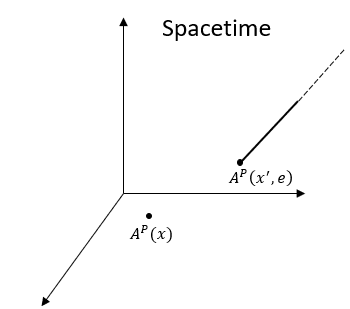
\includegraphics[width=0.25\textwidth]{1}
\end{wrapfigure}
Fields described in previous sections were all point-local. Operating $\partial_\mu$ on a p-loc field amounts to multiplying the intertwiners with $\pm ik_\mu$. Now one can ask, what can be the inverse operation for this? The answer to this question brings to a new kind of localization, the String Localization.

\begin{align*}
\int_{0}^{\infty} d s e^{-i p(x+s e)}=\lim _{\varepsilon \searrow 0} \frac{-i}{(p e)-i \varepsilon} \cdot e^{-i p x} \equiv \frac{1}{i(p e)_{-}} \cdot e^{-i p x}
\end{align*}
%(in the sense of distributions),
Integrating the field along a "string" $x+\mathbb{R}_{+} e$ multiplies the intertwiner with $\frac{-i}{(p e)_{-}}$. e is some spacelike direction and normalized, $e^{2}=-1$. We denote by $I_{e}$, the operation of string integration:
$$
\left(I_{e} \Phi\right)(x) \equiv \int_{0}^{\infty} d s\; \Phi(x+s e)
$$
One can see that $(e \partial) I_{e} \Phi=-\Phi,$ and hence, $I_{e}$ is minus the inverse of $(e \partial)=e^{\mu} \partial_{\mu}$.
$I_{e} \Phi$ is a string-local field.\\\\
From now on we will conceive the two-point function as ${}_m M^{X,Y}(p)$ for convenience. 
\begin{equation}
(\Omega, X(x) Y(y) \Omega)=\int \widetilde{d k}(p) \cdot e^{-i p(x-y)} \cdot {}_m M^{X, Y}(p)
\end{equation} 

\subsection{Spin 1}
Our spin 1 Proca field $A^P_\mu(x)$ is a p-loc field/potential which doesn't have a massless limit. This can be seen from 
\begin{align*}
{ }_{m} M^{A^P_{\mu}(x), A^P_{\nu}(x)}(p)=-\pi_{\mu\nu}(p)=-\eta_{\mu\nu}+\frac{p_\mu p_\nu}{m^2}
\end{align*} in the massless limit. But surely, the spin 1 field strength $F^P_{\mu\nu}(x)$, defined as the four-curl of $A^P_\mu(x)$, behaves well in the massless limit (\ref{eq:2.9}) ($\frac{p^\mu p^\nu}{m^2}$ term cancels due to the four-curl).\\\\
Using this field strength $F^P_{\mu\nu}(x)$, we define a s-loc field 

\begin{align}\label{eq:3.101}
A^P_{\mu}(x, e) &:=\left(I_{e} F^P_{\mu \nu}\right)(x) e^{\nu} \equiv \int_{0}^{\infty} d \lambda F^P_{\mu \nu}(x+\lambda e) e^{v} \\
a^P(x, e): &=-m^{-1} \partial^{\mu} A^P_{\mu}(x, e)\label{eq:3.102}.
\end{align}
The field $a^P(x,e)$ which accounts for the "Third State" simply decouples from the $A^P_\mu(x,e)$ as a massless scalar field $a(x,e)$ when taken the limit, refer equation (\ref{eq:3.104}). Both the fields (\ref{eq:3.101}) and (\ref{eq:3.102}) have well defined massless limit which can be seen from the two-point functions given below 
\begin{align}\label{eq:3.104}
&{ }_{m} M^{A^P_{\mu}(-e), A^P_{\nu}\left(e^{\prime}\right)}=-E\left(e, e^{\prime}\right)_{\mu \nu}(p)\\ &{}_m M^{a^P(-e), A^P_{\nu}\left(e^{\prime}\right)}=O(m), \quad{ }_{m} M^{a^P(-e), a^P\left(e^{\prime}\right)}=1+O\left(m^{2}\right),
\end{align}
where $E(e,e')$ is a distribution in $p$, $e$ and $e'$
\begin{align}
E\left(e, e^{\prime}\right)_{\mu \nu}(p):=\eta_{\mu v}-\frac{p_{\mu} e_{\nu}}{(p e)_{+}}-\frac{e_{\mu}^{\prime} p_{\nu}}{\left(p e^{\prime}\right)_{+}}+\frac{\left(e e^{\prime}\right) p_{\mu} p_{\nu}}{(p e)_{+}\left(p e^{\prime}\right)_{+}}.
\end{align}
At $m=0$, $A^P_\mu(x,e)$ becomes the massless s-loc vector potential $A_\mu(x,e)$ describing the Maxwell field strength, satisfying 
\begin{align}
\partial_\mu A_\nu(x,e)-\partial_\nu A_\mu(x,e)=F_{\mu\nu}(x).
\end{align}
One can prove it using the Jacobi identity.
Unlike $A^K_\mu(x)$ which does not exist on the Hilbert space, $A_\mu(x,e)$ lives on the Hilbert space as well, as it is derived from the gauge invariant operator $F_{\mu\nu}(x)$, alongside satisfying $e_\mu A^\mu(x,e)=0 $ and $\partial_\mu A^\mu(x,e)=0$.\\
On the Krein space, $A^K_\mu(x)$ and $A_\mu(x,e)$ are related to each other 
\begin{align}
A_\mu(x,e)=A^K_\mu(x)+\partial_\mu\varphi(x,e),\quad\text{where $\varphi(x,e)=\left(I_eA^K_\mu\right)(x)e^\mu$ is called the \textbf{\textcolor{blue!50!black}{ESCORT FIELD}},}
\end{align} 
but here $A_\mu(x,e)$ doesn't remain conserved anymore $\partial^\mu A_\mu(x,e)\neq0$, because $\partial^\mu A^K_{\mu}(x)\neq0$. \\\\
If we look at the transformation property of $A_\mu(x,e)$, the direction of the string e transforms along with the apex x.
\begin{align}\label{eq:3.7}
A_\mu(x,e)\longrightarrow\Lambda^\nu_{\;\mu}A_\nu(\Lambda x,\Lambda e).
\end{align}
This transformation property (\ref{eq:3.7}) explains why Coulomb gauge fails at Lorentz invariance. For $e=(1,\vec{0})$, $A^\mu(x,e)=(0,\vec{A}(x,e))$ coincides with the Coulomb gauge field $\vec{A}^{Cb}(x)$ with $A^0=0$. Since for the Coulomb gauge, e is fixed $(1,\vec{0})$, a Lorentz transformation might not keep this e fixed. \\
No Lorentz transformation can make two timelike strings into spacelike separated strings, implying the non-locality of $\vec{A}^{Cb}(x)$.    \\\\
Another way of looking at s-loc vector potentials is via the operator J defined as 
\begin{align}
J^\mu_{\;\nu}(e)&=\delta^\mu_{\;\nu}+\partial^\mu I_ee_\nu \label{eq:3.8}\\
&=\delta^\mu_{\;\nu}-\frac{p^\mu e_\nu}{(pe)_\pm}
\end{align}
and $A^P_\mu(x,e)=J^\nu_{\;\mu} A^P_\nu(x)$. Therefore one has the decomposition 
\begin{align*}
A_{\mu}^{\mathrm{P}}(x)&=\mathds{1}.A_{\mu}^{\mathrm{P}}(x)=\left(J^\nu_{\;\mu}-\partial_\mu I_e e^\nu\right)A_{\nu}^{\mathrm{P}}(x)\notag\end{align*}
\begin{align}
A_{\mu}^{\mathrm{P}}(x)=A^P_{\mu}(x, e)-m^{-1} \partial_{\mu} a^P(x, e), \quad m^{-1}a^P(x,e)=\varphi^P(e)=I_eA_{\nu}^{\mathrm{P}}(x)e^\nu.
\end{align}
So, one can reformulate QED in terms of string dependent Lagrangian L(e) by using $A^P(x)$ instead of indefinite Maxwell potential $A(x)$, couple it to a conserved current $j_\mu$ and take the massless limit. The massive escort field $a^P(x,e)$ carries away all the divergent pieces (explicit in $m^{-1}$) of $A^P(x)$ as m$\rightarrow 0$ as total derivatives leaving behind s-loc interaction Lagrangian $j_\mu A^\mu(x,e)$, which is renormalizable as well (UV dimension = 4).\\\\
Lastly, there also exists a massive vector potential $A^{K,m}_\mu(x)$ on the Krein space, of the same form as (\ref{eq:2.110}), with $p^0=\sqrt{m^2+\vec{p}^2}$. It converges to massless Krein potential $A^K_\mu(x)$ under the massless limit. \\\\
Various fields discussed in this section are compiled in the diagram below - 
\begin{figure}[H]
\centering
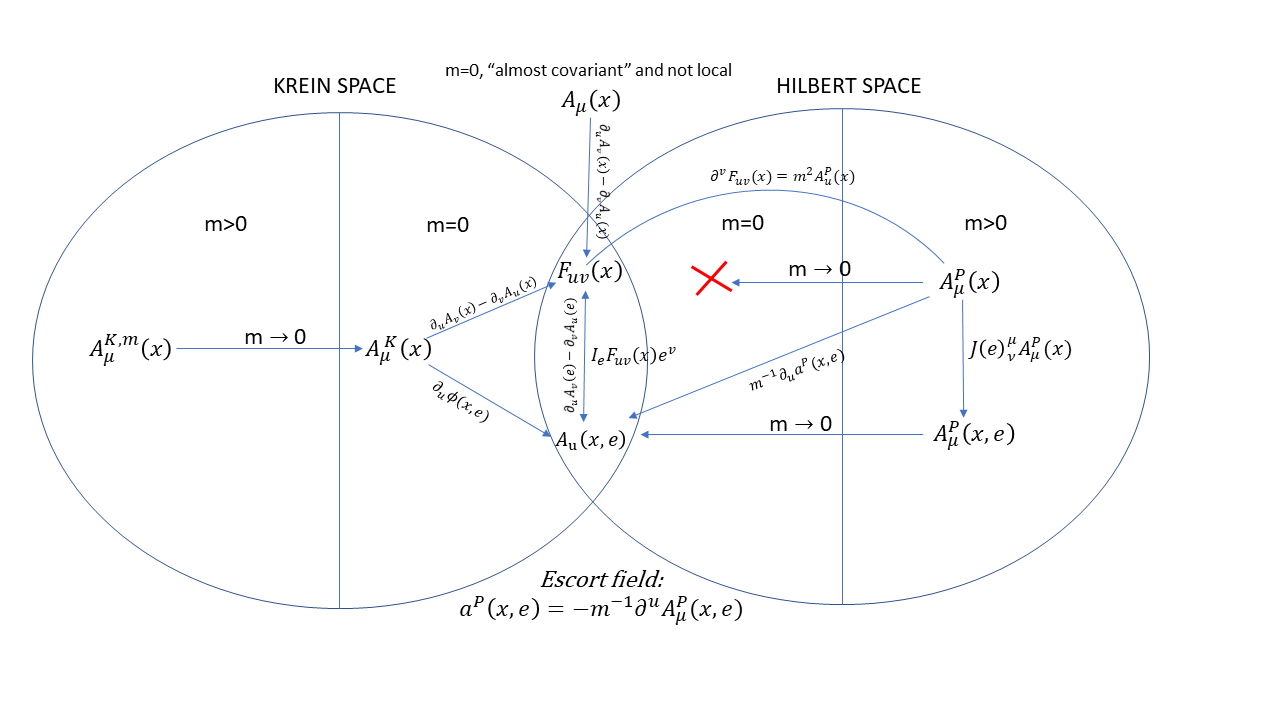
\includegraphics[scale=0.5]{s-lokal}
\caption{Spin 1 p-loc and s-loc vector potentials on Krein space and Hilbert space.}
\end{figure}    
\subsection{Spin 2}
Results from spin 1 case generalize to spin 2 as well. Here arises two additional features; The Weinberg–Witten theorem and the van Dam–Veltman–Zakharov discontinuity \cite{Mund_2017}\cite{2017NuPhB.924..699M}\cite{Zakharov:1970cc}\cite{VANDAM1970397}. We'll start this section by addressing the issue of DVZ discontinuity, looking at how it arises and analyse it in the s-loc setting. Consequence will be the $A^{(2)}_{\mu\nu}(x,e)$ field. 
\\\\
DVZ discontinuity is about the fact that, that in interacting models with spin$\geq2$, scattering amplitudes are discontinuous in the mass at $m=0$, i.e., the scattering of matter via exchange of  massless gravitons (say) is significantly different from the scattering by gravitons of a very small mass.    \\
The origin of this discontinuity can be found in the massless limit of  the spin 2 massive field strength $F^P_{\mu\nu}(x)$. 
\begin{align}
{ }_{m} M^{A_{\mu \nu}^{\mathrm{P}}(x), A_{\kappa \lambda}^{\mathrm{P}}(x)}&=\frac{1}{2}\left[\pi_{\mu \kappa} \pi_{\nu \lambda}+\pi_{\mu \lambda} \pi_{\nu \kappa}\right]-\frac{1}{3} \pi_{\mu \nu} \pi_{\kappa \lambda},
\\ \label{eq:3.1112}
{}_0 M^{A_{\mu \nu}^{\mathrm{F}}(x), A_{\kappa \lambda}^{\mathrm{F}}(x)}&=\frac{1}{2}\left[\eta_{\mu \kappa} \eta_{\nu \lambda}+\eta_{\mu \lambda} \eta_{\nu \kappa}\right]-\frac{1}{2} \eta_{\mu \nu} \eta_{\kappa \lambda}
\end{align}   
When taken the four-curl of $A^P(x)$ and $A^F(x)$ (massless Feynman gauge potential), the obtained two-point functions of the massive and massless field strengths differ by coefficients of `$-\frac{1}{3}$' and `$-\frac{1}{2}$' respectively. These coefficients are vestiges of having 5 physical one-particle subspaces and 2 physical one-particle subspaces associated to massive and massless field strength respectively. \\\\
Where's the discontinuity?
\begin{center}
$\underbrace{F^P_{[\mu \kappa][\nu \lambda]}(x)}_\text{-2,-1,0,+1,+2}\xrightarrow{m\rightarrow0}\underbrace{F_{[\mu \kappa][\nu \lambda]}(x)}_\text{-2,\textcolor{red}{0},+2}$
\end{center}
That spin 0 scalar field does not decouple dynamically from the $F_{[\mu \kappa][v \lambda]}$ (non-vanishing two point function), in a sense, it has to be removed `by hand', and hence the discontinuity. \\
With our s-loc field $A^{(2)}_{\mu\nu}(x,e)$ (modified $A^P_{\mu\nu}(x,e)$), things become a bit dynamic.    
\subsubsection{$\boldsymbol{A^P_{\mu\nu}(x,e)},\;m>0$}
Define \footnote{$A^P(x,e)$ and $A^P(e)$ are used interchangeably} - 
\begin{align}
A^P_{\mu v}(x, e)&=\left(I_{e}^{2} F^P_{[\mu \kappa][v \lambda]}\right)(x) e^{\kappa} e^{\lambda}=\int_{0}^{\infty}\int_{0}^{\infty} d \lambda d \lambda '\; F^P_{[\mu \kappa][v \lambda]}(x+\lambda e+\lambda 'e) e^{\kappa}e^\lambda\\&=\left(J_{e} \otimes J_{e}\right) A^{P}(x) 
\end{align}  
$A^P_{\mu v}(x, e)$ is the s-loc potential of the spin-2 Proca field strength, $J(e)$ has the definition (\ref{eq:3.8}). \\
\textbf{\textcolor{blue!50!black}{Escort fields} }
$$
\phi^P(x, e)=\left(\mathbf{1} \otimes I_{e} e\right) A^{P}(x)=\left(I_{e} e \otimes \mathbf{1}\right) A^{P}(x), \quad \varphi^P(x, e)=\left(I_{e} e \otimes I_{e} e\right) A^{P}(x)
$$
fill in 
\begin{align}\label{eq:3.11}
A^P_{\mu \kappa}(e)=A_{\mu \kappa}^{P}(x)+\left(\partial_{\mu} \phi^P_{\kappa}(e)+\partial^P_{\kappa} \phi_{\mu}(e)\right)+\partial_{\mu} \partial_{\kappa} \varphi^P(e).
\end{align}
$A^P_{\mu\nu}(x,e)$ is a potential. Above escort fields aren't well behaved. $\phi^P_{\mu}(e)$ and $\varphi^P$(e) have mass dimensions 0 and -1, carrying away all the singularities of $A^P(x)$ in the massless limit. 
We make well-behaved escort fields - 
$$
a^P_{\mu}(e)=-m^{-1} \partial^{\kappa} A^P_{\mu \kappa}(e)=m\left(\phi^P_{\mu}(e)+\partial_{\mu} \varphi^P(e)\right), \quad a^P(x, e)=-m^{-1} \partial^{\mu} a^P_{\mu}(e)=m^{2} \varphi^P(e)
$$
such that
\begin{align}
A_{\mu \nu}^{P}(x)=A^P_{\mu \nu}(e)-m^{-1}\left(\partial_{\mu} a^P_{\nu}(e)+\partial_{\nu} a^P_{\mu}(e)\right)+m^{-2} \partial_{\mu} \partial_{\nu} a^P(e).
\end{align}
$a^P_{\mu}(e)$ and $a^P(e)$ all have physical mass dimension $1,$ and have massless limits. Here, it's clear that all the singularities ($m^{-1}$ and $m^{-2}$ term) in the massless limit, fed inside $A^P(x)$, are being carried in the escort part.   \\
We're still not dynamic in helicity decouplings with this s-loc field because if we look at two-point functions 
\begin{flalign*}
&{}_m M^{A^P_{\mu v}(-e), A^P_{\kappa \lambda}\left(e^{\prime}\right)}=\frac{1}{2}\left[E\left(e, e^{\prime}\right)_{\mu \kappa} E\left(e, e^{\prime}\right)_{\nu \lambda}+(\kappa \leftrightarrow \lambda)\right]-\frac{1}{3} E(e, e)_{\mu \nu} E\left(e^{\prime}, e^{\prime}\right)_{\kappa \lambda}&\\&{ }_{0} M^{a_{\mu}^{P}(-e), a_{\nu}^{P}\left(e^{\prime}\right)}=-\frac{1}{2} E\left(e, e^{\prime}\right)_{\mu \nu}(p)&\\&{}_0 M^{a^P_\mu(-e), A^{P}_{\kappa\lambda}\left(e^{\prime}\right)}=0&\\&{}_0M^{a^P_\mu(-e), a^{P}\left(e^{\prime}\right)}=0&\\&
{}_0 M^{a^{P}(-e), A^P_{\mu \nu}\left(e^{\prime}\right)}=-\frac{1}{3} E\left(e^{\prime}, e^{\prime}\right)_{\mu v}(p)\longleftarrow\text{Semblance of DVZ discontinuity}& \\&
{}_0 M^{a^{P}(-e), a^{P}\left(e^{\prime}\right)}=\frac{2}{3}&
\end{flalign*} 
The fact that spin 0 scalar escort field $a^P(x,e)$ doesn't decouple from $A^P_{\kappa \lambda}\left(x,e\right)$ in the massless limit, is the origin of DVZ discontinuity. To cause this decoupling, we modify $A^P_{\kappa \lambda}\left(x,e\right)$, which brings us to the next section.
\subsubsection{$\boldsymbol{A^{(2)}_{\mu\nu}(x,e)},\;m>0$}

\begin{align}\label{eq:3.118}
A_{\mu \nu}^{(2)}(x, e)=A^P_{\mu \nu}(x, e)+\frac{1}{2} E(e, e)_{\mu \nu} a^P(x, e),
\end{align} where
$E(e, e)$ is the integro-differential operator
$$
E(e, e)_{\mu \nu}=\eta_{\mu \nu}+I_{e}\left(e_{\mu} \partial_{\nu}+e_{\nu} \partial_{\mu}\right)+e^{2} I_{e}^{2} \partial_{\mu} \partial_{\nu}
$$
involving two more string integrations. One can check that 
$$
\begin{array}{l}
{}_m M^{A_{\mu \nu}^{(2)}(-e), A_{\kappa \lambda}^{(2)}\left(e^{\prime}\right)}=\frac{1}{2}\left[E\left(e, e^{\prime}\right)_{\mu \kappa} E\left(e, e^{\prime}\right)_{\nu \lambda}+(\kappa \leftrightarrow \lambda)\right]-\frac{1}{2} E(e, e)_{\mu\nu} E\left(e^{\prime}, e^{\prime}\right)_{\kappa \lambda},
\end{array}
$$
and 
$$
{}_0 M^{a^{P}(-e), A^{(2)}_{\mu \nu}\left(e^{\prime}\right)}=0
$$
The coefficient `$-\frac{1}{2}$' of the last term matches with [3]. Thus, the massless limit of $A^{(2)}_{\mu\nu}(x, e)$ is the correct s-loc massless potential associated to a massless graviton.
$$
A_{\mu \nu}^{(2)}(x, e)=\left(I_{e}^{2} F_{[\mu \kappa][\nu \lambda]}^{(m=0)}\right)(x) e^{\kappa} e^{\lambda}
$$
\textbf{\textcolor{blue!50!black}{Properties of $A_{\mu \nu}^{(2)}(e)$ field}}-\\
It is symmetric, axial and satisfies 
\begin{align}\label{eq:3.1}
\eta^{\mu \nu} A_{\mu \nu}^{(2)}(e)=-\frac{m^{2}}{2} e^{2} I_{e}^{2} a^P(e)
\end{align} and 
\begin{align}\label{eq:3.2}
\partial^{\mu} A_{\mu \nu}^{(2)}(e)=-m a^P_{\nu}(e)-
\frac{m^{2}}{2} I_{e}(J e)_{\nu} a^P(e).
\end{align}
Staring at equation (\ref{eq:3.118}), one can ask if there is an s-loc massive field with less than four string integrations, also converging to the s-loc massless potential? Well, Yes. We call it $B^{(2)}_{\mu\nu}(x,e)$.

\subsubsection{$\boldsymbol{B^{(2)}_{\mu\nu}(x,e)},\;m>0$}
\footnote{Professor Rehren recently discovered this s-loc massive field $B^{(2)}_{\mu\nu}(x,e)$
that is
constructed from $A^P(x)$ with only two string integrations, and that also converges
to the correct s-loc massless potential. However, this field is not a potential, ie,
it does not differ from $A^P(x)$
by derivatives.}
\textbf{\textcolor{blue!50!black}{Construction of the $B^{(2)}_{\mu\nu}(x,e)$ field: } }
We start by considering the identity
$$
\partial_{\mu} \partial_{\nu} a^P(e)=m^{2} A_{\mu \nu}^{P}(x)+m\left(\partial_{\mu} a^P_{\nu}(e)+\partial_{\nu} a^P_{\mu}(e)\right)-m^{2} A^P_{\mu \nu}(e),
$$
where the last two terms are $O(m)$ and $O\left(m^{2}\right)$. Operating both sides with $-I_ee^{\mu}$ gives
$$
\partial_{\nu} a^P(e)=-m^{2} I_{e}\left(e A^{P}(x)\right)_{\nu}+m a^P_{\nu}(e),
$$
where the last term is $O(m)$. Operating with $-I_ee^{\nu}$ finally yields
$$
a^P(e)=m^{2} I_{e}^{2}\left(e A^{P}(x) e\right).
$$
Hence
\begin{align}\label{eq:3.3}
E(e, e)_{\mu \nu} a^P(e)=C_{\mu \nu}(e)+O(m),
\end{align}
where
$$
C_{\mu \nu}(e):=m^{2} I_{e}^{2}\left[\eta_{\mu \nu}\left(e A^{P}(x) e\right)-e_{\mu}\left(e A^{P}(x)\right)_{\nu}-\left(A^{P}(x) e\right)_{\mu} e_{\nu}+e^{2} A_{\mu \nu}^{P}(x)\right].
$$
The square bracket has the structure $e^{2} \Pi_{e}^{\perp} A^{P}(x) \Pi_{e}^{\perp}+\left(e A^{P}(x) e\right) \Pi_{e}^{\perp},$ where $\Pi_{e}^{\perp}=\mathds{1}-\frac{e.e}{e^2}$ is the (Lorentzian) projection orthogonal to $e .$ Hence the $B^{(2)}_{\mu\nu}(e)$ field 
\begin{align}\label{eq:3.4}
B_{\mu \nu}^{(2)}(e):=A^P_{\mu \nu}(e)+\frac{1}{2} C_{\mu \nu}(e).
\end{align}
Now taking the massless limit in (\ref{eq:3.3})
\begin{align*}
\lim_{m\rightarrow 0}\left(E(e, e)_{\mu \nu} a^P(e)=C_{\mu \nu}(e)\right)
\end{align*}
implying
\begin{align*}
\lim_{m\rightarrow o}\left(B_{\mu \nu}^{(2)}(e)=A_{\mu \nu}^{(2)}(e)\right).
\end{align*}
In words, $B_{\mu \nu}^{(2)}(e)$ field differs from $A_{\mu \nu}^{(2)}(e)$ by the discarded terms $O(m)$ and therefore has the same massless limit.  \\\\
\textbf{\textcolor{blue!50!black}{Properties of $B_{\mu \nu}^{(2)}(e)$}} - \\
Just like $A_{\mu \nu}^{(2)}(e), B_{\mu \nu}^{(2)}(e)$ is symmetric and axial. $B_{\mu \nu}^{(2)}(e)$ is exactly traceless. \\
It is not conserved, it follows
$$
\partial^{\mu} B_{\mu \nu}^{(2)}(e)=-\frac{m}{2} a^P_{\nu}(e).
$$
On comparison with (\ref{eq:3.1}) and (\ref{eq:3.2}), these properties look 'nicer'.  \\\\
\textbf{\textcolor{blue!50!black}{Intertwiners for $\boldsymbol{B^{(2)}_{\mu\nu}(x,e)}$ field}}-\\
To construct the intertwiners for the $B^{(2)}_{\mu\nu}(x,e)$ field, we borrow the known intertwiners of spin 2 p-loc Proca field (Appendix A).\\
We start from (\ref{eq:3.11}), and writing out the spin 2 Proca field under Weinberg-Wigner construction 
\begin{align}
(A^P)^{\mu\nu}(x)=\int \widetilde{dk}\left(U^{\mu\nu}_{ij}(k)a_{ij}(k)e^{-ikx}+h.c\right),    
\end{align}
where $U^{\mu\nu}_{ij}(k)$ are the known intertwiners of spin 2 Proca field. From (\ref{eq:3.4}) and (\ref{eq:3.11}), one can see that the intertwiners of the $B^{(2)}_{\mu\nu}(x,e)$ are related to the intertwiners of $(A^P)^{\mu\nu}(x)$ by partial derivatives and string integrations. \\
Intertwiners for $B^{(2)}_{\mu\nu}(x,e)$ reads 
\begin{align}
{}_{B}U^{\mu\nu}_{ij}(k)&=U^{\mu\nu}_{ij}(k)-\frac{1}{(ke)_-}\left(U^{\mu\kappa}_{ij}(k)e_\kappa k^\nu+U^{\nu\kappa}_{ij}(k)e_\kappa k^\mu\right)+\frac{1}{(ke)_-(ke)_-}\left[U^{\kappa\lambda}(k)e_\kappa e_\lambda k^\mu k^\nu\right.\notag\\&\left.\hspace{100pt}+\frac{m^2}{2}\left(\eta^{\mu\nu} U_{ij}^{\kappa\lambda}(k)e_\kappa e_\lambda-e^\mu e_\kappa U_{ij}^{\kappa\nu}(k)-U^{\mu\kappa}_{ij}(k)e_\kappa e^\nu+U^{\mu\nu}_{ij}(k)e^2\right)\right]
\end{align}
and 
${}_{B}U^{\mu\nu}_{ij}(k)={}_{B}\overline{U}^{\mu\nu}_{ij}(k)={}_{B}V^{\mu\nu}_{ij}(k)$ here.  \\
\\\\
Both $A^{(2)}_{\mu\nu}(x,e)$ and $B^{(2)}_{\mu\nu}(x,e)$ aren't potentials, in a sense that they do not differ from $A^P(x)$ by derivatives only. Whatever dynamics $A^{(2)}_{\mu\nu}(x,e)$ achieves in the massless limit, the same is achieved by $B^{(2)}_{\mu\nu}(x,e)$ with fewer (two) string integrations, also having `nicer' relations.  

\begin{figure}[H]
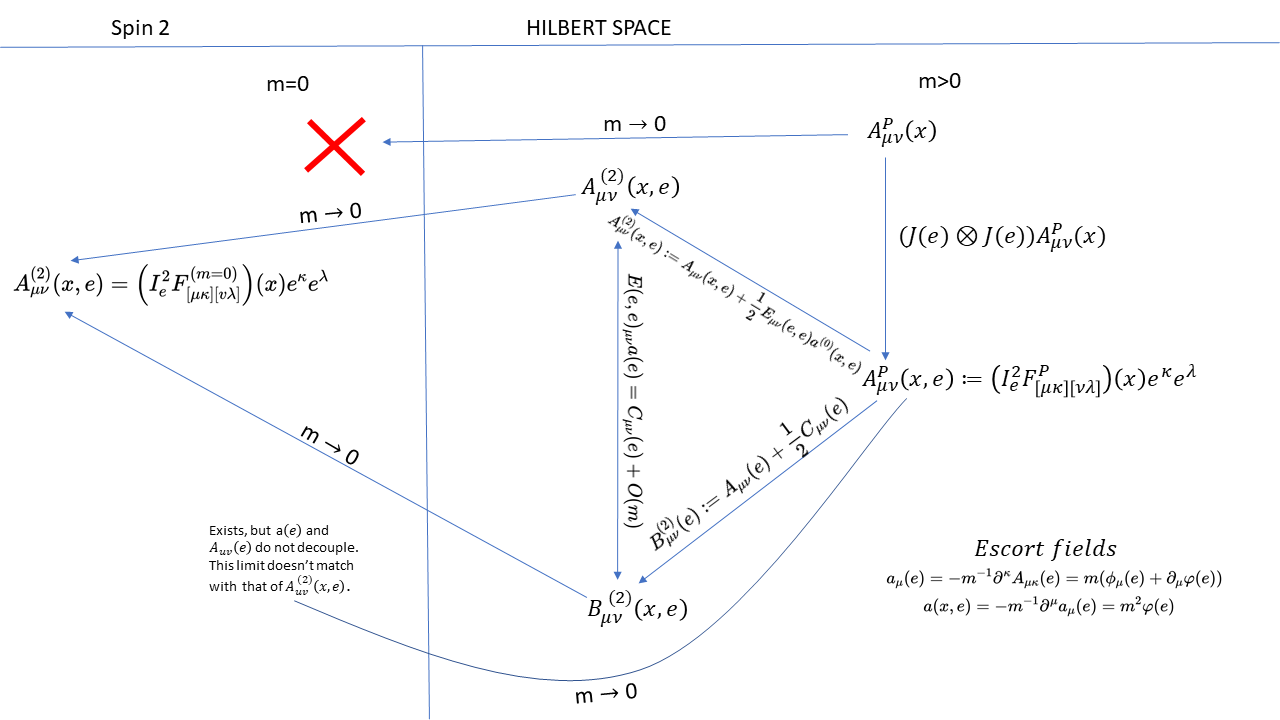
\includegraphics[scale=0.5]{2}
\caption{The spin 2 story}
\end{figure}


\subsection{Coupling of $\boldsymbol{A^{(2)}_{\mu\nu}(x,e)}$ and $\boldsymbol{B^{(2)}_{\mu\nu}(x,e)}$ field to matter fields}
\subsubsection{Aim and Theory}
This sections runs on this terrific fact that 'equations of motion don't change if we add total spacetime derivatives $\partial(\ddots)$ to the Lagrangian. \\\\
We don't have any string e dependence in the equations of motion of the fields known so far. So if we add any string dependence to the Lagrangian, say L(e), \textbf{\textcolor{blue!50!black}{its variation with respect to a string direction e should vanish,}}
\begin{align}
\frac{\partial L(e)}{\partial e^\kappa}=0 \quad \textbf{\textcolor{blue!50!black}{or}}\quad \frac{\partial Q^\mu_\kappa(e)}{\partial x^\mu}.
\end{align} 
Our \textbf{\textcolor{blue!50!black}{aim}} is to search for such $Q^\mu_\kappa(e)$'s composed of couplings of $\boldsymbol{A^{(2)}_{\mu\nu}(x,e)}$ and $\boldsymbol{B^{(2)}_{\mu\nu}(x,e)}$ field to matter fields/currents.
\subsubsection{The Problem}
Let's consider the field $B^{(2)}_{\mu\nu}(x,e)$ and some conserved current $T^{\mu\nu}(x)$. \\
String dependent Lagrangian $L(e)=B^{(2)}_{\mu\nu}(x,e)T^{\mu\nu}(x)$\\\\
Now
\begin{align}
\frac{\partial L(e)}{\partial e^\kappa}=&\left(\frac{\partial B^{(2)}_{\mu\nu}(x,e)}{\partial e^\kappa}\right)T^{\mu\nu}(x)+B^{(2)}_{\mu\nu}(x,e)\left(0\right)\notag\\
=&\left(\partial_\mu(X_{\kappa\nu})+\partial_\nu(Y_{\kappa\mu})+O(m)\right)T^{\mu\nu}(x).
\end{align} 
Upon partial integration and using $\partial_\mu T^{\mu\nu}(x)=0$
\begin{align}
\frac{\partial L(e)}{\partial e^\kappa}=O(m)T^{\mu\nu}(x) + \text{Total Derivatives}.
\end{align}
Therefore variation of action $S=\int d^4x\,\mathcal{L}(x,e)$ is \textbf{\textcolor{blue!50!black}{NOT}} string independent because $\frac{\delta S}{\delta e}=O(m)$. \\
Similar is the experience for $A^{(2)}_{\mu\nu}(x,e)$.
Anyhow, in the massless limit, this problem goes away. \\\\
Our \textbf{\textcolor{blue!50!black}{aim}} is to find suitable coupling candidates be it p-loc or s-loc, but they should exist.
\subsubsection{Candidate Hunt}
By looking at equations (\ref{eq:3.12}) and (\ref{eq:3.13}), one can make the following comments on the possible candidates for coupling to above modified s-loc spin 2 fields, and can narrow down on the choice of candidates - 
\begin{itemize}
\item
Since $A^{(2)}_{\mu\nu}(x,e)$ and $B^{(2)}_{\mu\nu}(x,e)$ are both symmetric, their coupling with any antisymmetric tensor will be trivial, or simply say, there's no coupling. Ex: Maxwell field strength tensor $F^{\mu\nu}(x)$,\\
\item
$A^{(2)}_{\mu\nu}(x,e)$ can couple with any conserved and traceless current/field. 
\item
$B^{(2)}_{\mu\nu}(x,e)$'s coupling like $\sim\eta^{\mu\nu} B^{(2)}_{\mu\nu}(x,e)$ is trivial, or basically no coupling, since $B^{(2)}_{\mu\nu}(x,e)$ is traceless.    
\item
Any current/field which is conserved, traceless, symmetric, and axial surely helps in being a possible candidate for coupling to $A^{(2)}_{\mu\nu}(x,e)$ and $B^{(2)}_{\mu\nu}(x,e)$.
\end{itemize} 
After all the build-up, we now look into some possible coupling candidates - \\\\
$COUPLING\; TO\; A^{(2)}_{\mu\nu}(x,e)\; FIELD$\\
\textbf{Candidates\footnote{These candidates fail to couple with $B^{(2)}_{\mu\nu}(x,e)$. It's a tough cookie to break.} : } 
\begin{enumerate}
\item
(A$^P)^{\mu\nu}(x)$. It is symmetric, traceless and conserved.
\begin{align}
L(e)&=A^{(2)}_{\mu\nu}(e)(A^P)^{\mu\nu}(x)
\end{align} 
\item
Stress energy tensor $T^{\mu\nu}(x)$ of - 
\begin{itemize}
\item Electromagnetic field
\item Massless Dirac field
\item Massless scalar field
\end{itemize}
are all symmetric, traceless and conserved. 
\begin{align}
L(e)&=A^{(2)}_{\mu\nu}(e)T^{\mu\nu}(x)
\end{align}
\end{enumerate}
$A^{(2)}_{\mu\nu}(e)$ forms a string-independent coupling with the above mentioned candidates (Appendix C for explicit calculation).\\\\
$COUPLING\; TO\; B^{(2)}_{\mu\nu}(x,e)\; FIELD$\\
For this field, I could find only \textbf{\textcolor{blue!50!black}{one candidate}}\footnote{Prof. Rehren - "Very interesting. It is something I had not expected.". Me - "Aaaaaaaaaaaaaaaa".}\\
\textbf{Candidate :}
\begin{align}\label{eq:3.15}
L(e)=\left(B^{(2)}_{\mu\nu}(e)-\frac{1}{2}m^2I_e^2e^2A^P_{\mu\nu}(x)\right)(A_0^{(2)}(e))^{\mu\nu}
\end{align}
where $(A^{(2)}_{0}(e))_{\mu\nu}$ is the massless, traceless, symmetric, axial and conserved s-loc spin 2 potential. \\
To arrive at above coupling, we start with - 
\begin{flalign}\label{eq:3.16}
\longrightarrow L(e)&=B^{(2)}_{\mu\nu}(e)(A^{(2)}_0(e))^{\mu\nu}+\underbrace{\left[-\frac{1}{m}\left(\partial_\mu a_\nu(e)+\partial_\nu a_\mu(e)\right)+\frac{1}{m^2}\partial_\mu\partial_\nu a(e)\right](A^{(2)}_0(e))^{\mu\nu}}_\textbf{Part A}\notag\\
&\hspace{250pt}-\underbrace{\frac{1}{2}\left[\eta_{\mu\nu}a(e)+m^2I_e^2e^2A^P_{\mu\nu}(x)\right](A^{(2)}_0(e))^{\mu\nu}}_\textbf{Part B} 
\end{flalign}
In Part A and Part B, one can perform partial integration and use the fact that $(A_0^{(2)}(e))^{\mu\nu}$ conserved and traceless to arrive at (\ref{eq:3.15}).\\
%\frac{\partial L(e)}{\partial e^\kappa}&=\frac{\partial B^{(2)}_{\mu\nu(e)}}{\partial e^\kappa}(A^{(2)}(e))^{\mu\nu}+B^{(2)}_{\mu\nu}(e)\frac{\partial (A^{(2)}(e))^{\mu\nu}}{\partial e^\kappa}\\
%&=\left(\partial_\mu\{I_e A(e)_{\kappa\nu}+\frac{1}{2}I_e E(e,e)_{\kappa\nu}a(e)+m[I_e^2(\frac{e_{\nu}a_\kappa(e)}{2}-(e_\kappa+e^2I_e\partial_\kappa)a_\nu(e))]\}\right.\\& \quad \left.+\partial_\nu\{\mu\longleftrightarrow\nu\}\right. \\&\left.\quad+\partial_\kappa\{ -\frac{mI_e^2}{2}[e_\mu a_\nu(e)+e_\nu a_\mu(e)]+m^2I_e^3e^2A_{\mu\nu}(e)\}\right.\\&\quad+\left.m[\eta_{\mu\nu}I_ea_k(e)-\frac{I_e}{2}(\eta_{\mu\kappa}a_\nu(e)+\eta_{\nu\kappa}a_\mu(e))]\right.\\&\quad+\left.m^2[I_e^2e_\kappa A_{\mu\nu}(e)-\frac{I_e^2}{2}(e_\mu A_{\kappa\nu}(e)+e_\nu A_{\kappa\mu}(e))]\right)(A^{(2)}(e))^{\mu\nu}+B^{(2)}_{\mu\nu}(e)\frac{\partial (A^{(2)}(e))^{\mu\nu}}{\partial e^\kappa}\\
%\end{flalign*}
%Using the fact that massless $(A^{(2)}(e))^{\mu\nu}$ is traceless, symmetric, conserved and axial, and also the relation $\eta^{\mu\nu}A_{\mu\nu}(e)=-a(e)$, we get, 
%\begin{flalign*}
%\quad&=\partial_\mu\underbrace{\left\lbrace \left(I_e A(e)_{\kappa\nu}+\frac{1}{2}I_e E(e,e)_{\kappa\nu}a(e)+m[I_e^2(\frac{e_{\nu}a_\kappa(e)}{2}-(e_\kappa+e^2I_e\partial_\kappa)a_\nu(e))]\right)(A^{(2)}(e))^{\mu\nu}\right\rbrace}_\textbf{X} \\
% &\quad +\partial_\nu\underbrace{\{(\mu\longleftrightarrow\nu)(A^{(2)}(e))^{\mu\nu}\}}_\textbf{Y}-m[\frac{I_e}{2}(\eta_{\mu\kappa}a_\nu(e)+\eta_{\nu\kappa}a_\mu(e))](A^{(2)}(e))^{\mu\nu}+B^{(2)}_{\mu\nu}(e)\frac{\partial (A^{(2)}(e))^{\mu\nu}}{\partial e^\kappa}\\
%& \quad =(\partial X)_\kappa+(\partial Y)_\kappa-m[\frac{I_e}{2}((A^{(2)}(e))\indices{_\kappa^\nu} a_\nu(e)+((A^{(2)}(e))\indices{_\kappa^\mu}a_\mu(e))]+B^{(2)}_{\mu\nu}(e)\frac{\partial (A^{(2)}(e))^{\mu\nu}}{\partial e^\kappa}
%\end{flalign*}
%Since for massless $A^{(2)}(e)$, $\partial_{e^\kappa}A^{(2)}_{\mu\nu}(e)=\partial_\mu I_e A^{(2)}_{\kappa\nu}(e)+\partial_\nu I_e A^{(2)}_{\kappa\mu}(e)$, also $\partial^\mu B^{(2)}_{\mu\nu}=-\frac{m}{2}a_\nu (e)$
%\begin{flalign*}
%&=(\partial X)_\kappa+(\partial Y)_\kappa\\
%&\quad-m[\frac{I_e}{2}((A^{(2)}(e))\indices{_\kappa^\nu} a_\nu(e)+((A^{(2)}(e))\indices{_\kappa^\mu}a_\mu(e))]+B^{(2)}_{\mu\nu}(e)\left(\partial^\mu I_e (A^{(2)}(e))\indices{_\kappa^\nu}+\partial^\nu I_e (A^{(2)}(e))\indices{_\kappa^\mu}\right)
%\end{flalign*}
%Upon partial integration - 
%\begin{flalign*}
%&=(\partial X)_\kappa+(\partial Y)_\kappa-m[\frac{I_e}{2}\cancel{((A^{(2)}(e))\indices{_\kappa^\nu} a_\nu(e)}+\cancel{((A^{(2)}(e))\indices{_\kappa^\mu}a_\mu(e))}]\\
%&\quad+\partial^\mu\left( B^{(2)}_{\mu\nu}(e) I_e (A^{(2)}(e))\indices{_\kappa^\nu}\right)+\partial^\nu \left( B^{(2)}_{\mu\nu}(e) I_e (A^{(2)}(e))\indices{_\kappa^\mu}\right)+\cancel{\frac{m}{2}I_e a_\nu(e)(A^{(2)}(e))\indices{_\kappa^\nu}}+\cancel{\frac{m}{2}I_e a_\mu(e)(A^{(2)}(e))\indices{_\kappa^\mu}}
%Therefore, variation of L(e) with respect to e is of total derivatives. No change to equations of motion. 
%\begin{flalign*}
%\frac{\partial L(e)}{\partial e^\kappa}=(\partial X)_\kappa+(\partial Y)_\kappa+\partial^\mu\left( B^{(2)}_{\mu\nu}(e) I_e (A^{(2)}(e))\indices{_\kappa^\nu}\right)+\partial^\nu \left( B^{(2)}_{\mu\nu}(e) I_e (A^{(2)}(e))\indices{_\kappa^\mu}\right)
%\end{flalign*}
Explicit breakdown of the candidate (\ref{eq:3.15}) forming a string-independent coupling can be found in Appendix C. 
\subsection{Stumbling over Haag's Theorem}
The coupling (\ref{eq:3.15}) is between a massive field(s) and a massless field. To analyze this, Prof. Rehren suggested to look at a much simpler case of coupling massive scalar fields A and B of mass $m_A$ and $m_B$ respectively.
\begin{align*}
L_A&=\frac{1}{2}\left(\partial_\mu A\partial^\mu A-m_A^2A^2\right)\\
L_B&=\frac{1}{2}\left(\partial_\mu B\partial^\mu B-m_B^2B^2\right)\\
L_{int}&=\mathcal{K} AB, \quad \text{$\mathcal{K}$ is the coupling constant}
\end{align*} 
Equations of motion - 
\begin{flalign}
\left(\square+m_B^2\right)B=\mathcal{K}A\quad \notag \\ 
\left(\square+m_A^2\right)A=\mathcal{K}B\quad \label{eq:3.34}
\end{flalign}
We then try to decouple the two fields A and B by writing the matrix equation - 
\begin{flalign}
\left(\square+M^2\right)C=0, \quad \text{where}\: C=\begin{pmatrix}
B\\A
\end{pmatrix} \text{and} \: M^2=\begin{pmatrix}
m^2_B&-\mathcal{K}\\-\mathcal{K}&m_A^2
\end{pmatrix} \quad \label{eq:3.35}
\end{flalign}
Now one can diagonalize the matrix $M^2$, the eigenvalues will be the masses $m_1$ and $m_2$ the decoupled fields \textbf{\textcolor{blue!50!black}{free}} $C_1$ and $C_2$ respectively,
\begin{align*}
m_1^2,\, m_2^2=\frac{(m_A^2+m_B^2)\pm\sqrt{(m_A-m_B)^2+4\mathcal{K}^2}}{2}
\end{align*}
and solve the matrix equation (\ref{eq:3.35}) to obtain $C_1(x)$ and $C_2(x)$. This sample AB coupling feels senseless as one of the masses can be negative for either $m_A=0$ or $m_B=0$, which is exactly the case (\ref{eq:3.15}).  \\\\
\textbf{\textcolor{blue!50!black}{The other obvious thing}} that would come in mind to solve equations (\ref{eq:3.34}) is via forming \textbf{\textcolor{blue!50!black}{convolutions in the Green's functions}} (something like a Born series). \\
Going through with this approach,
\begin{align*}
B(x)=B_0(x)-\int dy\int\frac{d^4k}{(2\pi)^4}\frac{e^{-ik(x-y)}\mathcal{K}A(y)}{k^2-m_B^2+i\epsilon}\\
A(y)=A_0(y)-\int dz\int\frac{d^4k}{(2\pi)^4}\frac{e^{-ik(y-z)}\mathcal{K}B(z)}{k^2-m_A^2+i\epsilon}
\end{align*}
Writing $\vartriangle_{m_B}(x-y)=\int\frac{d^4k}{(2\pi)^4}\frac{e^{-ik(x-y)}}{k^2-m_B^2+i\epsilon}$

\begin{align}\label{eq:3.335}
B(x)&=B_0(x)-\mathcal{K}\int dy\vartriangle_{m_B}(x-y)A_0(y)+\mathcal{K}^2\int\int dy \,dz \vartriangle_{m_B}(x-y)\vartriangle_{m_A}(y-z)B_0(z)\notag\\
&-\mathcal{K}^3\int\int\int dy\, dz\, dw \vartriangle_{m_B}(x-y)\vartriangle_{m_A}(y-z)\vartriangle_{m_B}(z-w)A_0(w)\notag\\
&+\mathcal{K}^4\int \int \int \int dy\, dz\, dw\, ds\, \vartriangle_{m_B}(x-y)\vartriangle_{m_A}(y-z)\vartriangle_{m_B}(z-w)\vartriangle_{m_A}(w-s)B_0(s)\notag\\
&-....
\end{align}
\textbf{\textcolor{blue!50!black}{Expectation}} from both the approaches was to get 'rotated' solutions, giving us \textbf{\textcolor{blue!50!black}{free}} fields $C_1(x)$ and $•C_2(x)$-
\begin{align}
C_1(x) = \cos(\alpha) B_0(x) - \sin(\alpha) A_0(x),\quad
C_2(x) = \sin(\alpha) B_0(x) + \cos(\alpha)A_0(x)
\end{align}
satisfying 
\begin{align}\label{eq:3.37}
(\square + m_1^2) C_1 = 0,\quad (\square +m^2_2)C_2 = 0\quad ....\textbf{but}
\end{align}
Now following the Haag's illustration \cite{Haag:212242} of \textbf{\textcolor{blue!50!black}{two neutral scalar fields of different masses}}, let $C_1(x)$ and $C_2(x)$ coincide at time $t=0$, $$C_1(\vec{x},0)=C_2(\vec{x},0)=C(\vec{x},0)$$ and corresponding conj. momentum $$\Pi_{C_1}(\vec{x},0)=\Pi_{C_2}(\vec{x},0)=\Pi_C(\vec{x},0)$$
The annihilation operator of $C_1(x)$ field $$a_{C_1}(\vec{k})=\sqrt{\omega_1(\vec{k})/2\hbar}\,C_1(\vec{k})+i\sqrt{1/2\hbar\omega_1(\vec{k})}\,\Pi_{C_1}(\vec{k}).$$
Annihilation operator of $C_2(x)$ is related to that of $C_1(x)$ by
\begin{align*}
a_{C_2}(\vec{k})=\frac{\omega_1+\omega_2}{2\sqrt{\omega_1\omega_2}}a_{C_1}(\vec{k})+\frac{\omega_2-\omega_1}{2\sqrt{\omega_1\omega_2}}a^*_{C_1}(\vec{k}).
\end{align*}
One can see that if 
\begin{align*}
a_{C_1}(\vec{k})\Omega=0\quad \text{where}\, \Omega\in\mathcal{H}\text{ is the vacuum state of the $C_1(x)$ field,}
\end{align*}
then $a_{C_2}(\vec{k})\Omega\neq0$. $C_2(x)$ is 'polarizing' the vacuum of the free theory of $C_1(x)$.
\textbf{\textcolor{blue!50!black}{This is the content of Haag's theorem.}}\\\\
\textbf{\textcolor{blue!50!black}{Professor Rehren}} \textbf{\textcolor{blue!50!black}{realized}} that while we use this Born series approach, it is also giving us \textbf{\textcolor{blue!50!black}{inequivalent representations}} of the commutator ring (\ref{eq:3.38}). Enter Haag's Theorem, which suggests - 
\begin{itemize}
\item There's no common Hilbert space representation for free and interacting field theories. 
\item The same is true for neutral \textbf{\textcolor{blue!50!black}{free}} \textbf{\textcolor{blue!50!black}{scalar}} fields of \textbf{\textcolor{blue!50!black}{different}} masses \cite{reed1975ii}.
\item Both $C_1(x)$ and $C_2(x)$ satisfy the (equal-time) CCR, \begin{align}\label{eq:3.38}
[\varphi(\vec{x}),\pi(\vec{x}')]=i\delta^{(3)}(\vec{x}-\vec{x}')
\end{align} But they don't live on the same Hilbert space. 
\item There is \textbf{\textcolor{blue!50!black}{no unitary transformation}} connecting $C_1(x)$ and $C_2(x)$.
\end{itemize}
\textbf{Comment on the issue of Haag's Theorem} - \\
Every time one does perturbation theory, he or she stumbles across Haag's Theorem. It isn't just brought into concern or conscious because the perturbation theory works fine, giving us predictions that match with the experiments. Yes, the Dyson series approach gives us inequivalent representations of the equal-time CCR. Writing a field in terms of some other field which doesn't share the same Hilbert space doesn't make sense. But then why does the approximations made in perturbation theory work? Well, 'this is because although Haag's theorem undercuts global unitary
equivalence, it is compatible with local unitary equivalence' \cite{pittphilsci2673}. According to Simon and Reed (1975) - 
\begin{adjustwidth}{50pt}{50pt}
Given any bounded region $B \subset \mathbb{R}^{3}$ and the free fields $\phi_{m_{1}}, \pi_{m_{1}}$ and $\phi_{m_{2}}, \pi_{m_{2}}$ acting on the respective Hilbert spaces $\mathcal{H}_{1}$ and $\mathcal{H}_{2}$, there is unitary map $V_{B}: \mathcal{H}_{1} \rightarrow \mathcal{H}_{2}$ such that $V_{B} \phi_{m_{1}}(f) V_{B}^{-1}=$
$\phi_{m_{2}}(f)$ and $V_{B} \pi_{m_{1}}(f) V_{B}^{-1}=\pi_{m_{2}}(f)$ for all suitable test functions $f$ with support in $B$. (p. 329)\\
\end{adjustwidth}
The issue of the perturbation series (\ref{eq:3.335}) being convergent or divergent has nothing to do with the Haag's Theorem. 
\section{SUMMARY}
The massive s-loc spin 2 field $A^{(2)}_{\mu\nu}(x,e)$  deals with the feature of DVZ discontinuity in a bit more dynamic fashion (causing decoupling of spin 0 scalar field and field strength in the massless limit, a vanishing two-point function). The same can be achieved by a field $B^{(2)}_{\mu\nu}(x,e)$ with only 2 string integrations. $B^{(2)}_{\mu\nu}(x,e)$ is traceless and have better looking spacetime derivatives. In the massless limit, these fields can be associated to $\pm2$ helicity state, describing a massless graviton. Hence, these  spin 2 string localized fields can be used to formulate coupling between massless (linearized) gravity and matter. \\\\
$A^{(2)}_{\mu\nu}(x,e)$ couples with any conserved matter field/current which is traceless and symmetric. It has more potential coupling candidates in comparison to $B^{(2)}_{\mu\nu}(x,e)$ field. For $B^{(2)}_{\mu\nu}(x,e)$, only one such L-Q pair was found which is  composed of something which is massive getting coupled to a massless spin 2 field $(A^{(2)}_0(x,e))^{\mu\nu}$, associated to massless graviton.\\
Analysis of the newly found coupling made us ponder upon the Haag's theorem, which states that there's no universal Hilbert representation describing both interacting and free fields. The same is true for neutral scalar fields of different masses.  
\newpage
\section{APPENDIX }
\begin{center}
\LARGE
\underline{\textbf{\textcolor{blue!50!black}{A}}}
\end{center}
\begin{center}

$\boldsymbol{FROM \, SPIN\, 1\, TO\, SPIN\, 2}$
\end{center}
\footnote{This appendix is typed and provided by Prof. Rehren.}The spin-1 ladder operators satisfy
$$
\left[a_{i}(p), a_{k}\left(p^{\prime}\right)^{*}\right]=(2 \pi)^{3} 2 p^{0} \delta_{i k} \delta\left(\vec{p}-\vec{p}^{\prime}\right)
$$
Therefore, ladder operators satisfying
$$
\left[\widetilde{a}_{i j}(p), \widetilde{a}_{k l}\left(p^{\prime}\right)^{*}\right]=(2 \pi)^{3} 2 p^{0} \delta_{i k} \delta_{j l} \delta\left(\vec{p}-\vec{p}^{\prime}\right)
$$
would create particles in the (spin-1 $\otimes$ spin-1) representation. One can project out the spin-2 subrepresentation by selecting the symmetric traceless part \footnote{This is true for any spin: The spin- $s$ subrepresentation of $(\operatorname{spin}-1)^{\otimes s}$ is the completely symmetric completely traceless part of $\left(\mathbb{R}^{3}\right)^{\otimes s}$.} :
$$
a_{i j}(p):=\Pi_{i j}^{i^{\prime} j^{\prime}} \widetilde{a}_{i^{\prime} j^{\prime}}(p)=\frac{1}{2}\left(\widetilde{a}_{i j}(p)+\widetilde{a}_{j i}(p)\right)-\frac{1}{3} \delta_{i j} \sum_{m} \widetilde{a}_{m m}(p)
$$
where
$$
\Pi_{i j}^{i^{\prime} j^{\prime}}=\frac{1}{2}\left(\delta_{i}^{i^{\prime}} \delta_{j}^{j^{\prime}}+\delta_{j}^{i^{\prime}} \delta_{i}^{j^{\prime}}\right)-\frac{1}{3} \delta^{i^{\prime} j^{\prime}} \delta_{i j}
$$
is the projection onto the symmetric traceless tensors. Consequently, there are exactly five linearly independent operators $a_{i j}(p)$.

One might pick a properly normalized basis $a_{I}(p)(I=1, \ldots, 5),$ which amounts to using Clebsch-Gordan coefficients. But it is more convenient (and perfectly equivalent) to work with this redundant system with linear dependences. The new commutations relations are
$$
\left[a_{i j}(p), a_{k l}\left(p^{\prime}\right)^{*}\right]=(2 \pi)^{3} 2 p^{0}\left[\frac{1}{2}\left(\delta_{i k} \delta_{j l}+\delta_{i l} \delta_{j k}\right)-\frac{1}{3} \delta_{i j} \delta_{k l}\right] \delta\left(\vec{p}-\vec{p}^{\prime}\right)
$$
Computing scalar products of states $a_{i j}(p)^{*}|0\rangle,$ one easily confirms that there are only five linearly independent states.

Correspondingly, we seek intertwiners with two Lorentz and two Euclidean indices $u_{i j}^{\mu \nu}(p) .$ For $p_{0},$ they are just given by $u_{0} \otimes u_{0} .$ There is no need for a projection, because they multiply the ladder operators that are already projected. But precisely for this reason, one may as well multiply $u_{0} \otimes u_{0}$ from the right with the projection operator $\Pi$, which has no effect when contracted with $a_{i j}$, but carries the information that $U$ can only be contracted with something traceless symmetric. Thus, the intertwiner for $A_{\mu \nu}^{P}$ is
$$
U_{i j}^{\mu \nu}(p)=\left(\Lambda_{p}\right)_{\mu^{\prime}}^{\mu}\left(\Lambda_{p}\right)_{\nu^{\prime}}^{\nu} u_{i^{\prime} j^{\prime}}^{\mu^{\prime} \nu^{\prime}}\left(p_{0}\right) \Pi_{i j}^{i^{\prime} j^{\prime}}=\left(\Lambda_{p}\right)_{i^{\prime}}^{\mu}\left(\Lambda_{p}\right)_{j^{\prime}}^{\nu} \Pi_{i j}^{i^{\prime} j^{\prime}}
$$
Trivially, $U_{i j}^{\mu \nu}(p)=U_{i j}^{\nu \mu}(p) .$ For the same reason as before, $p_{\mu} U_{i j}^{\mu \nu}(p)=0$ and $p_{\nu} U_{i j}^{\mu \nu}(p)=0 .$ Moreover,
$$
\eta_{\mu \nu} U_{i j}^{\mu \nu}(p)=\eta_{i^{\prime} j^{\prime}} \Pi_{i j}^{i^{\prime} j^{\prime}}=0
$$
because the range of $\Pi$ is traceless. These identities secure the symmetry, conservation and tracelessness of the spin- 2 Proca field.
\newpage
\begin{center}
\LARGE
\underline{\textbf{\textcolor{blue!50!black}{B}}}
\end{center}
\begin{center}
$\boldsymbol{DERIVATIVES\, OF\, S\text{-}LOC\, FIELDS}$
\end{center}
\begin{flalign}
&\frac{\partial A^P_{\mu\nu}(e)}{\partial e^\kappa}=\partial_\mu (I_eA^P_{\kappa\nu}(e))+(\mu\longleftrightarrow\nu)&
\end{flalign}
\begin{flalign}\label{eq:3.12}
&\frac{\partial A^{(2)}_{\mu\nu}(e)}{\partial e^\kappa}=\partial_\mu\left\lbrace A^P(e)_{\kappa\nu}+\frac{1}{2}I_e E(e,e)_{\kappa\mu}a^P(e)+m\left[I_e^2\left(e_\nu+\frac{I_e e^2\partial_\nu}{2}\right)a^P_\kappa(e)\right]\right\rbrace\notag\\& \hspace{45pt}+\{\mu\longleftrightarrow\nu\}+m(\eta_{\mu\nu}I_ea^P_k(e))&
\end{flalign}
\begin{flalign} \label{eq:3.13}
&\frac{\partial B^{(2)}_{\mu\nu}(e)}{\partial e^\kappa}=\partial_\mu\left\lbrace I_e A^P(e)_{\kappa\nu}+\frac{1}{2}I_e E(e,e)_{\kappa\nu}a^P(e)+m\left[I_e^2\left(\frac{e_{\nu}a^P_\kappa(e)}{2}-\left(e_\kappa+e^2I_e\partial_\kappa\right)a^P_\nu(e)\right)\right]\right\rbrace\notag\\& \hspace{45pt} +\left\lbrace\mu\longleftrightarrow\nu\right\rbrace\notag \\&\hspace{45pt}+\partial_\kappa\left\lbrace -\frac{mI_e^2}{2}\left[e_\mu a^P_\nu(e)+e_\nu a^P_\mu(e)\right]+m^2I_e^3e^2A^P_{\mu\nu}(e)\right\rbrace\notag\\&\hspace{45pt}+m\left[\eta_{\mu\nu}I_ea^P_k(e)-\frac{I_e}{2}(\eta_{\mu\kappa}a^P_\nu(e)+\eta_{\nu\kappa}a^P_\mu(e))\right]\notag\\&\hspace{45pt}+m^2\left[I_e^2e_\kappa A^P_{\mu\nu}(e)-\frac{I_e^2}{2}(e_\mu A^P_{\kappa\nu}(e)+e_\nu A^P_{\kappa\mu}(e))\right]&
\end{flalign}
Above $\frac{\partial B^{(2)}_{\mu\nu}}{\partial e^\kappa}$ has 5 string integrations. Writing the derivative in this fashion has the advantage of having the powers m being explicit. \\Though it can also be written in terms of 3 string integrations. 
\begin{align}
&\frac{\partial B^{(2)}_{\mu\nu}(e)}{\partial e^\kappa}=\partial_\mu \left\lbrace I_e(A^P_{\kappa\mu}(x)+\partial_\kappa I_e(eA^P)_\nu(x)+\partial_\nu I_e(A^P(x)e)_\kappa+\partial_\kappa\partial_\nu I_e^2(eA^P(x)e))\right\rbrace+(\mu\longleftrightarrow\nu)\notag\\&\hspace{50pt} +\partial_\kappa\{I_eC_{\mu\nu}(e)\}+\frac{1}{2}m^2I_e^2\left[2\eta_{\mu\nu}(A^P(x)e)_\kappa-\delta_{\mu\kappa}(eA^P(x))_\nu-e_\mu A^P_{\kappa\nu}(x)-A^P_{\mu\kappa}(x)e_\nu\notag\right.\\&\left.\hspace{45pt}\hspace{250pt}-(A^P(x)e)_\mu\delta_{\nu\kappa}\hspace{10pt}+2e_\kappa A^P_{\mu\nu}(x)\right]&
\end{align}
\newpage

\begin{center}
\LARGE
\underline{\textbf{\textcolor{blue!50!black}{C}}}
\end{center}

\begin{center}
$\boldsymbol{COUPLING\, TO\, A^{(2)}_{\mu\nu}(x,e)\, FIELD}$
\end{center}
\begin{flalign*}
1.\longrightarrow L(e)&=A^{(2)}_{\mu\nu}(e)(A^P)^{\mu\nu}(x)\\
\frac{\partial L(e)}{\partial e^\kappa}&=\frac{\partial A^{(2)}_{\mu\nu(e)}}{\partial e^\kappa}(A^P)^{\mu\nu}(x)+A^{(2)}_{\mu\nu}(e)\frac{\partial (A^P)^{\mu\nu}(x)}{\partial e^\kappa}\\
&=\partial_\mu\{I_e A(e)_{\kappa\nu}+\frac{1}{2}I_e E(e,e)_{\kappa\mu}a(e)+m[I_e^2(e_\nu+\frac{I_e e^2\partial_\nu}{2})a_\kappa(e)]\}(A^P)^{\mu\nu}(x)\\& \quad+\partial_\nu\{\mu\longleftrightarrow\nu\}(A^P)^{\mu\nu}(x)+m(\eta_{\mu\nu}I_ea_k(e))(A^P)^{\mu\nu}(x)+0
\end{flalign*}
Since $(A^P)^{\mu\nu}(x)$ is traceless and conserved, $\eta_{\mu\nu}(A^P)^{\mu\nu}(x)=0$ and $\partial_\mu (A^P)^{\mu\nu}(x)=0$, variation of L(e) w.r.t e is a total derivative of spacetime.
\begin{align*}
\frac{\partial L(e)}{\partial e^\kappa}&=\partial_\mu\left\lbrace \left(I_e A^P(e)_{\kappa\nu}+\frac{1}{2}I_e E(e,e)_{\kappa\mu}a^P(e)+m[I_e^2(e_\nu+\frac{I_e e^2\partial_\nu}{2})a^P_\kappa(e)]\right)(A^P)^{\mu\nu}(x)\right\rbrace \\& \quad+\partial_\nu\left\lbrace \left(\mu\longleftrightarrow\nu\right)(A^P)^{\mu\nu}(x)\right\rbrace +0
\end{align*}
Similarly, $A^{(2)}_{\mu\nu}(e)$ couples with other candidates. \\
\begin{center}
$\boldsymbol{COUPLING\, TO\, B^{(2)}_{\mu\nu}(x,e)\, FIELD}$
\end{center}
\textbf{Breakdown:} Starting with (\ref{eq:3.16})
\begin{flalign*}
L(e)&=\left[A^P_{\mu\nu}(e)+\frac{1}{2}C_{\mu\nu}(e)\right](A^{(2)}_0(e))
+\underbrace{\left[-\frac{1}{m}\left(\partial_\mu a^P_\nu(e)+\partial_\nu a^P_\mu(e)\right)+\frac{1}{m^2}\partial_\mu\partial_\nu a^P(e)\right](A^{(2)}_0(e))^{\mu\nu}}_\textbf{Part A}\\
&\hspace{270pt}-\underbrace{\frac{1}{2}\left[\eta_{\mu\nu}a^P(e)+m^2I_e^2e^2A^P_{\mu\nu}(x)\right](A^{(2)}_0(e))^{\mu\nu}}_\textbf{Part B}\\
\end{flalign*}
Combining Part A with $A_{\mu\nu}(e)$ and Part B with $C_{\mu\nu}(e)$, while using the expressions - 
\begin{align*}
&A^P_{\mu\nu}(x)=A^P_{\mu\nu}(e)-m^{-1}\left(\partial_\mu a^P_\nu (e)+\partial_\nu a^P_\mu(e)\right)+m^{-2}\partial_\mu\partial_\nu a^P(e)&\\
&C_{\mu\nu}(e)-\underbrace{m^2I_e^2\eta_{\mu\nu}(eA^P(x)e)}_\textbf{$\eta_{\mu\nu}a(e)$}-m^2I_e^2e^2A^P_{\mu\nu}(x)=m^2I_e^2[-e_\mu(eA^P(x))_\nu-(A^P(x)e)_\mu e_\nu]
\end{align*}
L(e) reduces to - 
\begin{flalign*}
L(e)=\left(A^P_{\mu\nu}(x)-\frac{1}{2}m^2I_e^2\left[e_\mu(eA^P(x))_\nu+(A^P(x)e)_\mu e_\nu\right]\right)(A^{(2)}_0(e))^{\mu\nu}
\end{flalign*}
Since $(A^{(2)}_0(e))^{\mu\nu}$ is axial and symmetric -\\ 
\begin{align*}
L(e)=A^P_{\mu\nu}(x)(A^{(2)}_0(e))^{\mu\nu}
\end{align*}
and, 
\begin{align*}
\frac{\partial L(e)}{\partial e^\kappa}&=\partial^\mu\left( A^P_{\mu\nu}(x) I_e (A^{(2)}_0(e))\indices{_\kappa^\nu}\right)+\partial^\nu \left( A^P_{\mu\nu}(x) I_e (A^{(2)}_0(e))\indices{_\kappa^\mu}\right).
\end{align*}

\newpage
\textbf{Comments and Ideas:}
\begin{itemize}
\item Haag's theorem says that the fields of mass m and m' don't share the same fock space, the same ground state. I have to find a relation between the ground states of their respective Fock spaces, and in the weak limit show that the inner product (of their respective ground state) goes to 0. 
\item Idea 1: Can't we write the ground state of mass m free field in expansion some expansion of cutoff basis.
\item Idea 2: Prof. Rehren's idea of rescaling the fields - diffeos.
\item Idea 3: Identifying time 0 fields, and writing creation and annihilation operators of mass m field in terms of other field of mass m'. 
\item Prof. Rehren's idea has similarity to some work done  here - \url{https://arxiv.org/abs/1001.0946}{}
\end{itemize}

\newpage
\bibliographystyle{unsrt}
\bibliography{Bibliography}


\end{document}



